\runningheader{Oppgave c)}{}{Side \thepage\ av \numpages}

% ********************************************************
% oppgave c) 
% ********************************************************  
\item
  Kopier modellen fra a) og bygg den som vist under, hvor initialverdien til integratoren er $y(0){=}0$.
  \begin{figure}[H]
    \centering
    \hspace*{0mm}\scalebox{0.8}{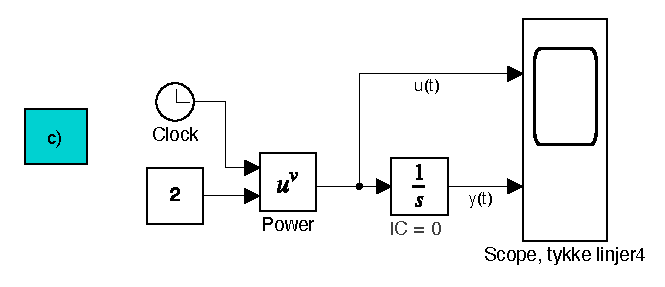
\includegraphics{2c.pdf}}
  \end{figure}
  
  {\color{red}La simuleringstiden fortsatt være 25 sekund.}

    {\bf Svar på følgende spørsmål:    }

  \begin{enumerate}[label=c\arabic*)]
    \item   Hva er det analytiske uttrykket for $u(t)$ som er modellert?
    \item Hva blir det analytiske uttrykket for $y(t)$?
    \item Simuler modell og ta med simuleringsresultatet i
      innleveringen din ved å bruke prosedyren på
     side~\pageref{page:prosedyre}.

\item Vis/forklar at simuleringsresultatet  stemmer
  overens med  det analytiske uttrykket for $y(t)$. 
  
  \end{enumerate}
